%%%%%%%%%%%%%%%%%%%%%%%%%%%%%%%%%%%%%%%%%%%%%%%%%%%%%%%%%%%%%%%%%%%%%%%%%%%%%%%
%                         File: osa-revtex4-1.tex                             %
%                        Date: April 15, 2013                                 %
%                                                                             %
%                              BETA VERSION!                                  %
%                   JOSA A, JOSA B, Applied Optics, Optics Letters            %
%                                                                             %
%            This file requires the substyle file osajnl4-1.rtx,              %
%                   running under REVTeX 4.1 and LaTeX 2e                     %
%                                                                             %
%                   USE THE FOLLOWING REVTeX 4-1 OPTIONS:                     %
% \documentclass[osajnl,twocolumn,showpacs,superscriptaddress,10pt]{revtex4-1}%
%                    %% Use 11pt for Applied Optics                           %
%                                                                             %
%               (c) 2013 The Optical Society of America                       %
%                                                                             %
%%%%%%%%%%%%%%%%%%%%%%%%%%%%%%%%%%%%%%%%%%%%%%%%%%%%%%%%%%%%%%%%%%%%%%%%%%%%%%%

\documentclass[osajnl,twocolumn,showpacs,superscriptaddress,10pt]{revtex4-1} %% use 11pt for Applied Optics
%\documentclass[osajnl,preprint,showpacs,superscriptaddress,11pt]{revtex4-1} %% use 12pt for preprint option
\usepackage{amsmath,nccmath,amssymb,graphicx,float,minted,xparse,tikz}
\usepackage[utf8]{inputenc}
\graphicspath{{images/}}

\usepackage{mathtools,enumitem}
\usepackage{minted}

\begin{document}

\title{Programación Distribuida y Tiempo Real}

\author{Ulises Jeremias Cornejo Fandos}
\affiliation{Licenciatura en Informática, Facultad de Informática, UNLP}

\maketitle %% required

\section{Para los ejemplos de RPC proporcionados (*.tar, analizar en el orden dado a los nombres de
los archivos):}

\subsection{Mostrar cómo serían los mismos procedimientos si fueran locales, es decir haciendo el
proceso inverso del realizado en la clase de explicación de RPC.}

Si los procesos fueran todos locales, la programación de los mismos resultaria en una compilación de uno o más ".c" con una única función \textit{main} y un único binario ejecutable. En el ejemplo provisto se puede observar como todo el código del programa se encuentra en un único ".c", como se describe anteriormente.

En este caso no habría latencia en la comunicación dado que no existiría tal comunicacón. Al no definirse un modelo cliente/servidor, ya no existiría una comunicación entre hosts y todos los llamados a funciones se realizarían en el mismo espacio de direcciones.

\subsection{Ejecutar los procesos y mostrar la salida obtenida (del “cliente” y del “servidor”) en cada
uno de los casos.}

Las capturas se muestran a continuación:

\subsubsection{Simple}

\begin{figure}[H]
    \centering
    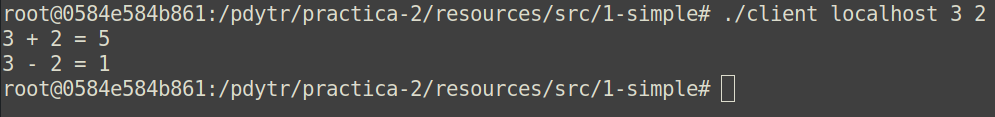
\includegraphics[width=0.5\textwidth]{capturas/1-simple-client}
    \caption{Salida de la ejecución del cliente dados los parámetros \textit{localhost}, \textit{3} y \textit{2}}.
    \label{figure:1-simple-client}
\end{figure}

\begin{figure}[H]
    \centering
    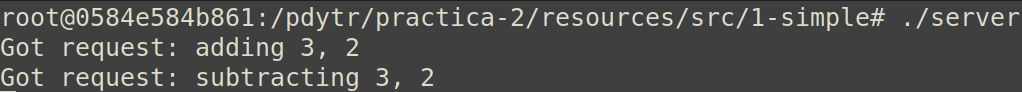
\includegraphics[width=0.5\textwidth]{capturas/1-simple-server}
    \caption{Salida de la ejecución del servidor.}
    \label{figure:1-simple-server}
\end{figure}

\subsubsection{U1}

La ejecución del servidor no tiene salida al momento de resolver una consulta del cliente.

\begin{figure}[H]
    \centering
    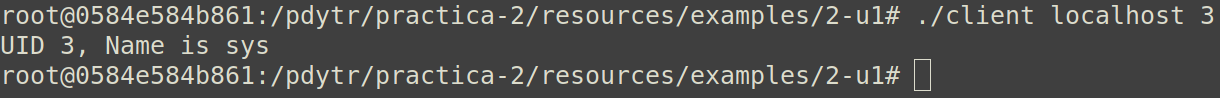
\includegraphics[width=0.5\textwidth]{capturas/2-u1-client}
    \caption{Salida de la ejecución del cliente dados los parámetros \textit{localhost} y \textit{3}}.
    \label{figure:2-u1-client}
\end{figure}

\subsubsection{Array}

\begin{figure}[H]
    \centering
    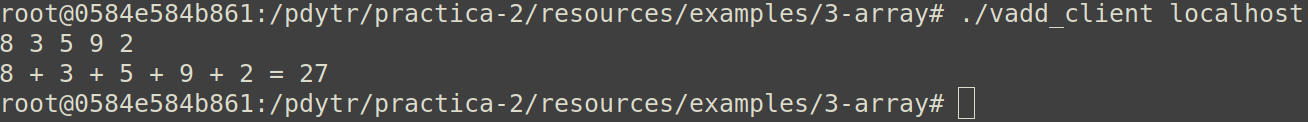
\includegraphics[width=0.5\textwidth]{capturas/3-array-client}
    \caption{Salida de la ejecución del cliente dados los parámetros \textit{localhost}, $8$, $3$, $5$, $9$ y $2$}.
    \label{figure:3-array-client}
\end{figure}

\begin{figure}[H]
    \centering
    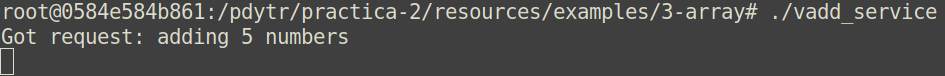
\includegraphics[width=0.5\textwidth]{capturas/3-array-server}
    \caption{Salida de la ejecución del servidor.}
    \label{figure:3-array-server}
\end{figure}

\subsubsection{List}

La ejecución del servidor no tiene salida al momento de resolver una consulta del cliente.

\begin{figure}[H]
    \centering
    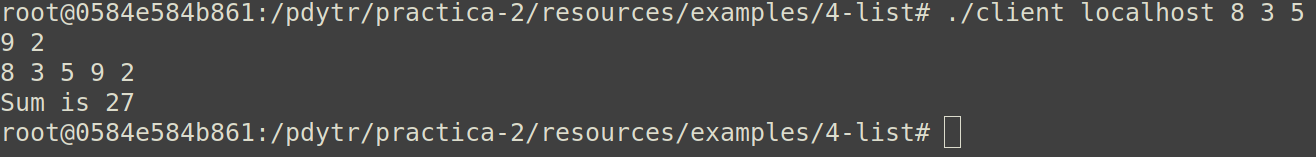
\includegraphics[width=0.5\textwidth]{capturas/4-list-client}
    \caption{Salida de la ejecución del cliente dados los parámetros \textit{localhost}, $8$, $3$, $5$, $9$ y $2$}.
    \label{figure:4-list-client}
\end{figure}

\subsection{Mostrar experimentos donde se produzcan errores de conectividad del lado del cliente y
del lado del servidor. Si es necesario realice cambios mínimos para, por ejemplo, incluir
sleep() o exit(), de forma tal que no se reciban comunicaciones o no haya receptor para
las comunicaciones. Verifique con UDP y con TCP.}

En ambos casos se modifica la implementación de la función \mintinline{c}{int *add_1_svc(operands *argp, struct svc_req *rqstp);} en el archivo \textit{simpservice.c}. Es decir, la implementación del proceso servidor, agregando un sleep o exit, según corresponda, respectivamente.

\subsubsection{UDP}
  Agregando un llamado a la función \textbf{exit}, el proceso servidor termina en medio de la operación, (\textit{ver fig. \ref{figure:1-simple-server-udp-exit}}) por lo que el cliente termina la comunicación cuando finaliza el timeout definido en su proceso, (\textit{ver fig. \ref{figure:1-simple-client-udp-exit}}).
  
  Lo mismo pasa si el servidor tarda mucho en procesar lo pedido y responder, cosa que se simula agregando un llamadao a la función \textbf{sleep} dentro del proceso servidor. Cuando el sleep tiene una duración mayor a la del timeout definido en el cliente, el servidor no da su respuesta antes del timeout y el cliente cierra la conexión, (\textit{ver fig. \ref{figure:1-simple-client-udp-sleep}}). En este caso, el servidor continuará su ejecución esperando el proximo request, (\textit{ver fig. \ref{figure:1-simple-server-udp-sleep}}).
  
\begin{figure}[H]
    \centering
    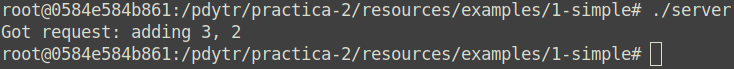
\includegraphics[width=0.5\textwidth]{capturas/1-simple-server-udp-exit}
    \caption{Salida de la ejecución del service utilizando UDP y la función exit.}.
    \label{figure:1-simple-server-udp-exit}
\end{figure}

\begin{figure}[H]
    \centering
    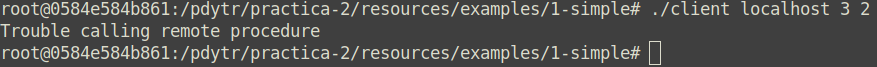
\includegraphics[width=0.5\textwidth]{capturas/1-simple-client-udp-exit}
    \caption{Salida de la ejecución del cliente utilizando UDP.}.
    \label{figure:1-simple-client-udp-exit}
\end{figure}

\begin{figure}[H]
    \centering
    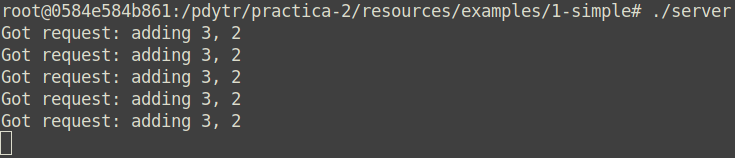
\includegraphics[width=0.5\textwidth]{capturas/1-simple-server-udp-sleep}
    \caption{Salida de la ejecución del service utilizando UDP y la función sleep.}.
    \label{figure:1-simple-server-udp-sleep}
\end{figure}

\begin{figure}[H]
    \centering
    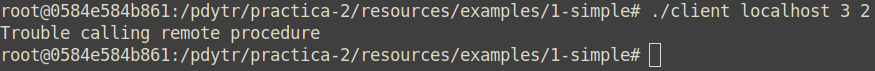
\includegraphics[width=0.5\textwidth]{capturas/1-simple-client-udp-sleep}
    \caption{Salida de la ejecución del cliente utilizando UDP.}.
    \label{figure:1-simple-client-udp-sleep}
\end{figure}

\subsection{TCP}

El resultado es exactamente el mismo que el descripto anteriormente en el caso de UDP, cuando el servidor termina cuando se agrega el \textbf{exit}, (\textit{ver figs. \ref{figure:1-simple-server-tcp-exit} y \ref{figure:1-simple-client-tcp-exit}}) y cuando tarda mas de lo debido con la función \textbf{sleep}, (\textit{ver figs. \ref{figure:1-simple-server-tcp-sleep} y \ref{figure:1-simple-client-tcp-sleep}}).

\begin{figure}[H]
    \centering
    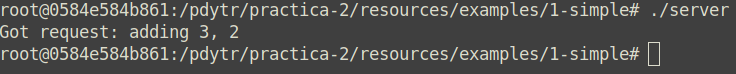
\includegraphics[width=0.5\textwidth]{capturas/1-simple-server-tcp-exit}
    \caption{Salida de la ejecución del service utilizando TCP y la función exit.}.
    \label{figure:1-simple-server-tcp-exit}
\end{figure}

\begin{figure}[H]
    \centering
    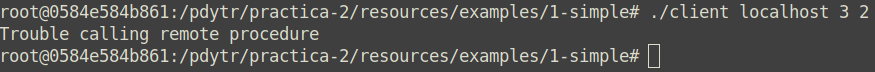
\includegraphics[width=0.5\textwidth]{capturas/1-simple-client-tcp-exit}
    \caption{Salida de la ejecución del cliente utilizando TCP.}.
    \label{figure:1-simple-client-tcp-exit}
\end{figure}

\begin{figure}[H]
    \centering
    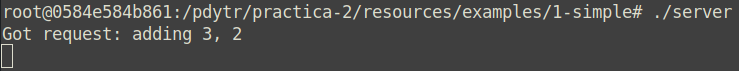
\includegraphics[width=0.5\textwidth]{capturas/1-simple-server-tcp-sleep}
    \caption{Salida de la ejecución del service utilizando TCP y la función sleep.}.
    \label{figure:1-simple-server-tcp-sleep}
\end{figure}

\begin{figure}[H]
    \centering
    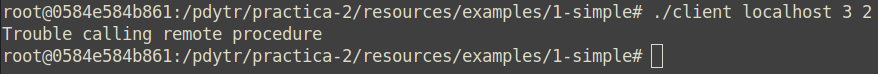
\includegraphics[width=0.5\textwidth]{capturas/1-simple-client-tcp-sleep}
    \caption{Salida de la ejecución del cliente utilizando TCP.}.
    \label{figure:1-simple-client-tcp-sleep}
\end{figure}

\section{Describir/analizar las opciones a) - N b) -M y - A, verificando si se pueden utilizar estas opciones y comentar que puede ser necesario para tener procesamiento concurrente del “lado del cliente” y del “lado del servidor” con la versión
utilizada de rpcgen. Una lista completa de opciones se describe en
http://download.oracle.com/docs/cd/E19683-01/816-1435/rpcgenpguide-1939/index.html}

\subsection{}
El flag -N intenta de generar código en un estándar más nuevo que el ANSI (flag -C).
Al intentar compilar el código con ese flag, utilizando el código original, falla.
Esto se debe a que rcpgen, genera un .h las funciones con el tipo SIN puntero, a diferencia del flag -C, que los genera como punteros a operand.

\subsection{}
El flag -M sirve para generar código seguro para la concurrencia, utilizando un paŕametro extra al servicio, de tipo int *. \\
El flag -A, es la configuracion por default, que dependiendo el sistema en el que se compila, va a ser (o no), seguro para la concurrencia multihilo.

\section{Analizar la transparencia de RPC en cuanto al manejo de parámetros de los procedimientos
remotos. Considerar lo que sucede en el caso de los valores de retorno. Puede aprovechar los
ejemplos provistos.}

rpcgen utiliza la estructura definida en el archivo ".x" para generar estructuras C en ambos puntos (cliente y servidor), con las cuales va a trabajar casteando. \\

El servicio recibe punteros a estas estructuras, las cuales va a trabajar y retornar nuevamente casteando a (caddr\_t), el cual es equivalente a un \mintinline{c}{void *}.

Esto nos permite trabajar con cualquier tipo de C, siempre volviendo a castear a la estructura definida a partir del ".x".

\end{document}
